% Options for packages loaded elsewhere
\PassOptionsToPackage{unicode}{hyperref}
\PassOptionsToPackage{hyphens}{url}
\documentclass[
]{article}
\usepackage{xcolor}
\usepackage{amsmath,amssymb}
\setcounter{secnumdepth}{-\maxdimen} % remove section numbering
\usepackage{iftex}
\ifPDFTeX
  \usepackage[T1]{fontenc}
  \usepackage[utf8]{inputenc}
  \usepackage{textcomp} % provide euro and other symbols
\else % if luatex or xetex
  \usepackage{unicode-math} % this also loads fontspec
  \defaultfontfeatures{Scale=MatchLowercase}
  \defaultfontfeatures[\rmfamily]{Ligatures=TeX,Scale=1}
\fi
\usepackage{lmodern}
\ifPDFTeX\else
  % xetex/luatex font selection
\fi
% Use upquote if available, for straight quotes in verbatim environments
\IfFileExists{upquote.sty}{\usepackage{upquote}}{}
\IfFileExists{microtype.sty}{% use microtype if available
  \usepackage[]{microtype}
  \UseMicrotypeSet[protrusion]{basicmath} % disable protrusion for tt fonts
}{}
\makeatletter
\@ifundefined{KOMAClassName}{% if non-KOMA class
  \IfFileExists{parskip.sty}{%
    \usepackage{parskip}
  }{% else
    \setlength{\parindent}{0pt}
    \setlength{\parskip}{6pt plus 2pt minus 1pt}}
}{% if KOMA class
  \KOMAoptions{parskip=half}}
\makeatother
\usepackage{longtable,booktabs,array}
\newcounter{none} % for unnumbered tables
\usepackage{calc} % for calculating minipage widths
% Correct order of tables after \paragraph or \subparagraph
\usepackage{etoolbox}
\makeatletter
\patchcmd\longtable{\par}{\if@noskipsec\mbox{}\fi\par}{}{}
\makeatother
% Allow footnotes in longtable head/foot
\IfFileExists{footnotehyper.sty}{\usepackage{footnotehyper}}{\usepackage{footnote}}
\makesavenoteenv{longtable}
\usepackage{graphicx}
\makeatletter
\newsavebox\pandoc@box
\newcommand*\pandocbounded[1]{% scales image to fit in text height/width
  \sbox\pandoc@box{#1}%
  \Gscale@div\@tempa{\textheight}{\dimexpr\ht\pandoc@box+\dp\pandoc@box\relax}%
  \Gscale@div\@tempb{\linewidth}{\wd\pandoc@box}%
  \ifdim\@tempb\p@<\@tempa\p@\let\@tempa\@tempb\fi% select the smaller of both
  \ifdim\@tempa\p@<\p@\scalebox{\@tempa}{\usebox\pandoc@box}%
  \else\usebox{\pandoc@box}%
  \fi%
}
% Set default figure placement to htbp
\def\fps@figure{htbp}
\makeatother
\setlength{\emergencystretch}{3em} % prevent overfull lines
\providecommand{\tightlist}{%
  \setlength{\itemsep}{0pt}\setlength{\parskip}{0pt}}
\usepackage{bookmark}
\IfFileExists{xurl.sty}{\usepackage{xurl}}{} % add URL line breaks if available
\urlstyle{same}
\hypersetup{
  hidelinks,
  pdfcreator={LaTeX via pandoc}}

\author{}
\date{}

\begin{document}

\section{Paper 12: The Twin Minimal Space
Model}\label{paper-12-the-twin-minimal-space-model}

\subsection{External Face of the Stable Species, the Exact Form of
Measurement, Layer Resolution of Entanglement, and Vertex Deficits with
Two Hidden Axes --- Interface Emergence of Quantum-Like
Behavior}\label{external-face-of-the-stable-species-the-exact-form-of-measurement-layer-resolution-of-entanglement-and-vertex-deficits-with-two-hidden-axes-interface-emergence-of-quantum-like-behavior}

Author: Noriaki Kihara\\
Affiliation: WF System Co., Ltd.\\
ORCID: 0009-0004-6753-4020\\
Version: v0.2\\
Date: June 2026\\
DOI (this version): 10.5281/zenodo.20640469\\
Concept DOI: 10.5281/zenodo.20640468\\
License: CC BY 4.0

\begin{center}\rule{0.5\linewidth}{0.5pt}\end{center}

\subsection{Abstract}\label{abstract}

As the final paper of the series, this paper constructs the minimal
system in which two composites coexist --- the \textbf{twin minimal
space model} --- and examines how much of the behavior that looks
quantum mechanical is derived as a \textbf{reading of hierarchy
interfaces} in a discrete relational model that assumes neither
amplitudes nor continuous time.

\textbf{External face of the stable species}: The handles (hairs) by
which a composite is observed from outside divide into three ledgers:
the face fundamental wave \(\nu_0=1/(2\sqrt s)\) (the dominant line of
the self-container spectrum), the parent-record line
\(\nu_{\mathrm{obs}}=|k|\), and the energy-like norm \(R'=\sqrt s\). The
exact identity \(\nu_0 R'=1/2\) (the zero point) links the first two,
and \(R'\) never appears as a line --- it is readable from outside
\textbf{as the spacing \(1/R'\) of the odd comb} (the particle-level
realization of the record theorem). The external face is a
\textbf{minimal-uncertainty quasi-rectangular wave packet} that carries
a built-in odd comb of spacing \(1/R'\) and is localized within an
extent \(2R'\) (half-width × fundamental wave = \(1/2\)).

\textbf{Construction of the twin system}: The initial value
\(\Omega_0^2=2\nu_1^2=18\) is an even label and, by the classification
theorem (Paper 5), cannot exist as a single state --- \textbf{being born
as a pair is forced by parity} (the first event requires no dynamics).
The allowed lattice separations of the twins (each \(s=9\)) are
quantized to \(|\Delta|^2\in\{2,\ldots,20\}\), and
\(|\Delta|^2\equiv1\pmod4\) is entirely forbidden. The 18 relational
classes are completely separated by fringe data alone --- \textbf{the
scale marks of space are born as chord sets of equal-frequency shells}.

\textbf{The exact form of measurement}: Inspecting the two conditions
for measurement (affecting the system; detecting the change), the
detection of change requires knowledge of the prior state and regresses
infinitely; in this model, however, the record of the prior state is
absent by censorship, and the \(\lambda\) ledger is append-only (the
monotonic increase theorem, Paper 6), so the regress is structurally
cut. \textbf{Measurement = an append to the record (absence →
presence)}; ``collapse'' is the appearance of a record, and its
irreversibility reduces to the same single bit as the arrow of time.
Computing the first decay of the twins explicitly, the appearance of the
reference wave (\(s=1\)) promotes the information class of the record
from interferometric to holographic --- \textbf{the measuring apparatus
is generated by the event itself}. We also show that the final-state
statistics depend on the choice of measure (one-shot equal weight over
configurations \(60/61\) versus sequential conditional counting
\(396/403\)) --- \textbf{measure bifurcation}, with an exact difference
of \(+0.00098\).

\textbf{Layer resolution of entanglement}: The self-spectrum of a single
fragment lies on all-components-even vectors and is therefore
identically invisible in the logical-wave (odd) sector --- \textbf{only
counts and relations can be read} (the relational-only readout theorem).
The decay of one twin instantaneously rewrites the branching statistics
of the other (total variation 0.774), but this shift \textbf{does not
depend on the twin separation at all}, and the influence does not
propagate through the space of the child layer --- instantaneity is not
a speed but a mismatch of levels. Since order and attribution do not
exist in the final record, operational no-signalling follows. An
entangled pair, being an even label, cannot become a single particle at
the layer above (parity protection). The same map applies to two-path
interference of a single wave packet.

\textbf{Vertex deficits and the two hidden axes}: An exhaustive
inspection of the record continuity rule across an event (that the
parent's identity line persists in the cross spectrum of the daughter
system) \textbf{derives, as the persistence condition, a conservation
law of position vectors \(v_5\pm v_3=\pm v_9\) (a momentum analogue)},
which holds for parents in the \((2,1,0,0)\) orbit but fails for parents
in the \((1,1,1,1)\) orbit by \textbf{exactly one unit} (one axis / one
quantum). Furthermore, in the bookkeeping of the excitation degree
\(\varepsilon=(-1)^{\Sigma|k|}\) there exists a second one-bit deficit
\textbf{independent} of this one (specific orbits at \(s=7,9\)). The
visible four-axis ledgers demand two invisible directions --- R on the
curvature side and Q on the bare-parity side --- and intermediate
displacements along the invisible directions, being unrecorded, are
permitted (\textbf{the licensing principle for virtual displacements}).
This licence virtually unlocks two-body splittings that are forbidden in
the visible ledgers, and \textbf{decomposes every decay into sequences
of cubic vertices} (multiple paths to the same final state).

Finally, we organize the correspondence between the obtained structure
and standard theory as a \textbf{transport principle} (a theorem is
transported whenever the counterparts of its premises are verified), and
state explicitly the candidate answers this model gives to questions
that remain postulates on the standard-theory side (the measurement
problem, the location of the cut, the problem of time, dimensionality,
the measure), together with falsifiability (gravitationally mediated
entanglement experiments, etc.).

\begin{center}\rule{0.5\linewidth}{0.5pt}\end{center}

\subsection{Keywords}\label{keywords}

composite particle, wave packet, relational observables, measurement
problem, no-signalling, entanglement, Bell inequalities, virtual states,
hidden dimensions, Kaluza--Klein, structural correspondence

\begin{center}\rule{0.5\linewidth}{0.5pt}\end{center}

\subsection{1. Introduction}\label{introduction}

The point of arrival of the series (Papers 5--11 {[}2{]}), built upon
the reciprocal dual model (introduced up to Paper 4 {[}1{]}), was that a
discrete, timeless, amplitude-free relational model possesses discrete
spectra, an uncertainty floor, exclusion statistics, gauge structure,
and dimensional selection as theorems. The question of this paper is the
final step:

\begin{quote}
Of the behaviors held to be peculiar to quantum mechanics --- wave
packets, the irreversibility of measurement, the nonlocal correlations
of entanglement, virtual states --- how much is derived as a
\textbf{reading of hierarchy interfaces} of this model, and from where
on is essentially new input required?
\end{quote}

There are two methodological keys. First, to use \textbf{the minimal
two-body system}: twins with equal representative frequencies remove the
unresolved clock problem from the setting and leave only purely
relational observables. Second, to take \textbf{the record} as the
consistent arbiter: an observable is a recordable quantity (Paper 6).

Related context: the measurement problem and the measurement chain (von
Neumann {[}5{]}), the emergence of classicality via decoherence (Zurek
{[}6{]}), Bell's theorem and the CHSH inequality {[}7,8{]}, the
gravity-induced state reduction hypothesis (Penrose {[}9{]}) and
experimental proposals for gravitationally mediated entanglement (Bose
et al.~{[}10{]}, Marletto \& Vedral {[}11{]}), virtual intermediate
states in the path integral (Feynman {[}12{]}), charge from extra
dimensions (Kaluza {[}13{]}, Klein {[}14{]}), and information-based
viewpoints (Wheeler {[}4{]}). This paper is not an extension of these
theories; it is an inspection of how far the exhaustive computation of a
finite model reproduces their \textbf{structure}.

\begin{center}\rule{0.5\linewidth}{0.5pt}\end{center}

\subsection{2. External Face of the Stable Species: Three Ledgers and
the Wave
Packet}\label{external-face-of-the-stable-species-three-ledgers-and-the-wave-packet}

\subsubsection{2.1 Three representative frequencies and the
identity}\label{three-representative-frequencies-and-the-identity}

There are three handles by which the stable species \(s=1,3,5\) (Paper
7) are observed from outside (by exact computation of the self-container
spectrum):

{\def\LTcaptype{none} % do not increment counter
\begin{longtable}[]{@{}
  >{\raggedright\arraybackslash}p{(\linewidth - 8\tabcolsep) * \real{0.1667}}
  >{\raggedleft\arraybackslash}p{(\linewidth - 8\tabcolsep) * \real{0.2222}}
  >{\raggedleft\arraybackslash}p{(\linewidth - 8\tabcolsep) * \real{0.2222}}
  >{\raggedleft\arraybackslash}p{(\linewidth - 8\tabcolsep) * \real{0.2222}}
  >{\raggedright\arraybackslash}p{(\linewidth - 8\tabcolsep) * \real{0.1667}}@{}}
\toprule\noalign{}
\begin{minipage}[b]{\linewidth}\raggedright
Quantity
\end{minipage} & \begin{minipage}[b]{\linewidth}\raggedleft
\(s=1\)
\end{minipage} & \begin{minipage}[b]{\linewidth}\raggedleft
\(s=3\)
\end{minipage} & \begin{minipage}[b]{\linewidth}\raggedleft
\(s=5\)
\end{minipage} & \begin{minipage}[b]{\linewidth}\raggedright
Status
\end{minipage} \\
\midrule\noalign{}
\endhead
\bottomrule\noalign{}
\endlastfoot
Face fundamental wave \(\nu_0=1/(2\sqrt s)\) & 0.5000 & 0.2887 & 0.2236
& Dominant line of the self-container spectrum \\
Parent-record line \(\nu_{\mathrm{obs}}=\lvert k\rvert\) & 0 (DC) & 1 &
\(\sqrt2\) & Line appearing in the parent's unit record \\
Norm \(R'=\sqrt s\) & 1 & 1.732 & 2.236 & Conservation ledger.
\textbf{Never appears as a line} \\
\end{longtable}
}

The exact identity \(\nu_0R'=1/2\) (the zero point) links the face
ledger and the norm ledger. \(\nu=\sqrt s\) falls on the even rungs of
the face ladder and does not exist in the odd spectrum --- the
energy-like quantity is read not as the position of a line but as
\textbf{the spacing \(1/R'\) of the odd comb} (that is, as an extension
quantity on the \(\lambda\) side). This is the particle-level
realization of the record theorem (Paper 6: \(\nu\) is recorded only as
a \(\lambda\) configuration). Note that a pure odd comb occurs only for
\(s=1\); a composite \textbf{signs its compositeness to the outside} as
the parity contamination rate of the comb (49\% for \(s=3\), 21\% for
\(s=5\)).

\subsubsection{2.2 The external face as a wave
packet}\label{the-external-face-as-a-wave-packet}

The external face is a quasi-rectangular solitary wave packet that (i)
is localized within a finite extent \(2R'\), (ii) self-restores exactly
with period \(2R'\) thanks to the commensurate odd comb, and (iii)
saturates the \textbf{minimal uncertainty} half-width × fundamental wave
= \(1/2\). The mechanism that preserves the shape is not nonlinearity
but censorship (Paper 9). The energy label is estimated from the lines
of the parent record via the zero-point dressing formula
\(s=\nu_{\mathrm{obs}}^2+\|k\|_1+1\).

\begin{figure}
\centering
\pandocbounded{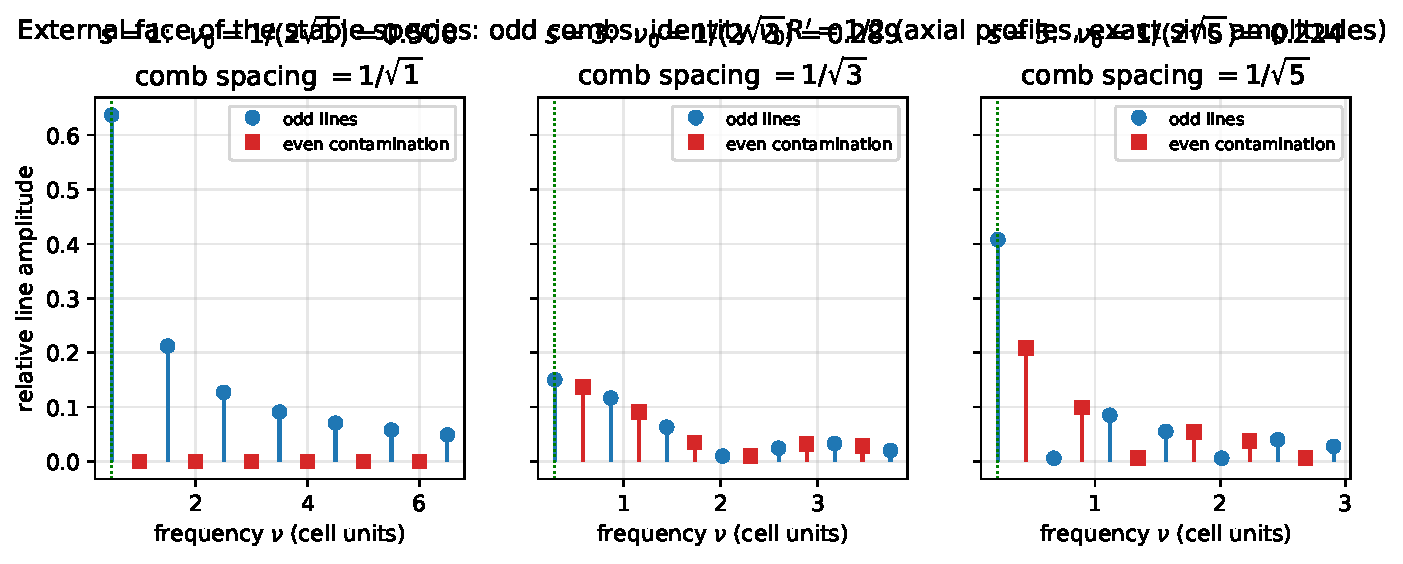
\includegraphics[keepaspectratio,alt={Figure 1. External face of the stable species: odd combs}]{figure_paper12_1_species_combs.pdf}}
\caption{Figure 1. External face of the stable species: odd combs}
\end{figure}

\textbf{Figure 1. External face of the stable species (exact sinc
amplitudes of an axis section): the odd-comb spacing \(1/\sqrt s\)
conveys \(R'\), and the contamination rate of even lines conveys
compositeness, to the outside. Green dotted line = face fundamental wave
\(\nu_0=1/(2\sqrt s)\).}

\begin{center}\rule{0.5\linewidth}{0.5pt}\end{center}

\subsection{3. The Twin Minimal Space
Model}\label{the-twin-minimal-space-model}

\subsubsection{3.1 Pair creation forced by
parity}\label{pair-creation-forced-by-parity}

Consider a system that initially possesses only a single oscillation
frequency \(\Omega_0\), and set up the situation in which it splits into
two \(s=9\) composites under the conservation law
\(\Omega_0^2=2\nu_1^2=18\). \(S=18\) is even and, by the classification
theorem (Paper 5), \textbf{has no single-state slot}. On the d=4
lattice, therefore, the option of remaining single does not
kinematically exist for this system --- it does not ``break apart'' but
is \textbf{born as a pair}. The first event requires no dynamics.

\begin{figure}
\centering
\pandocbounded{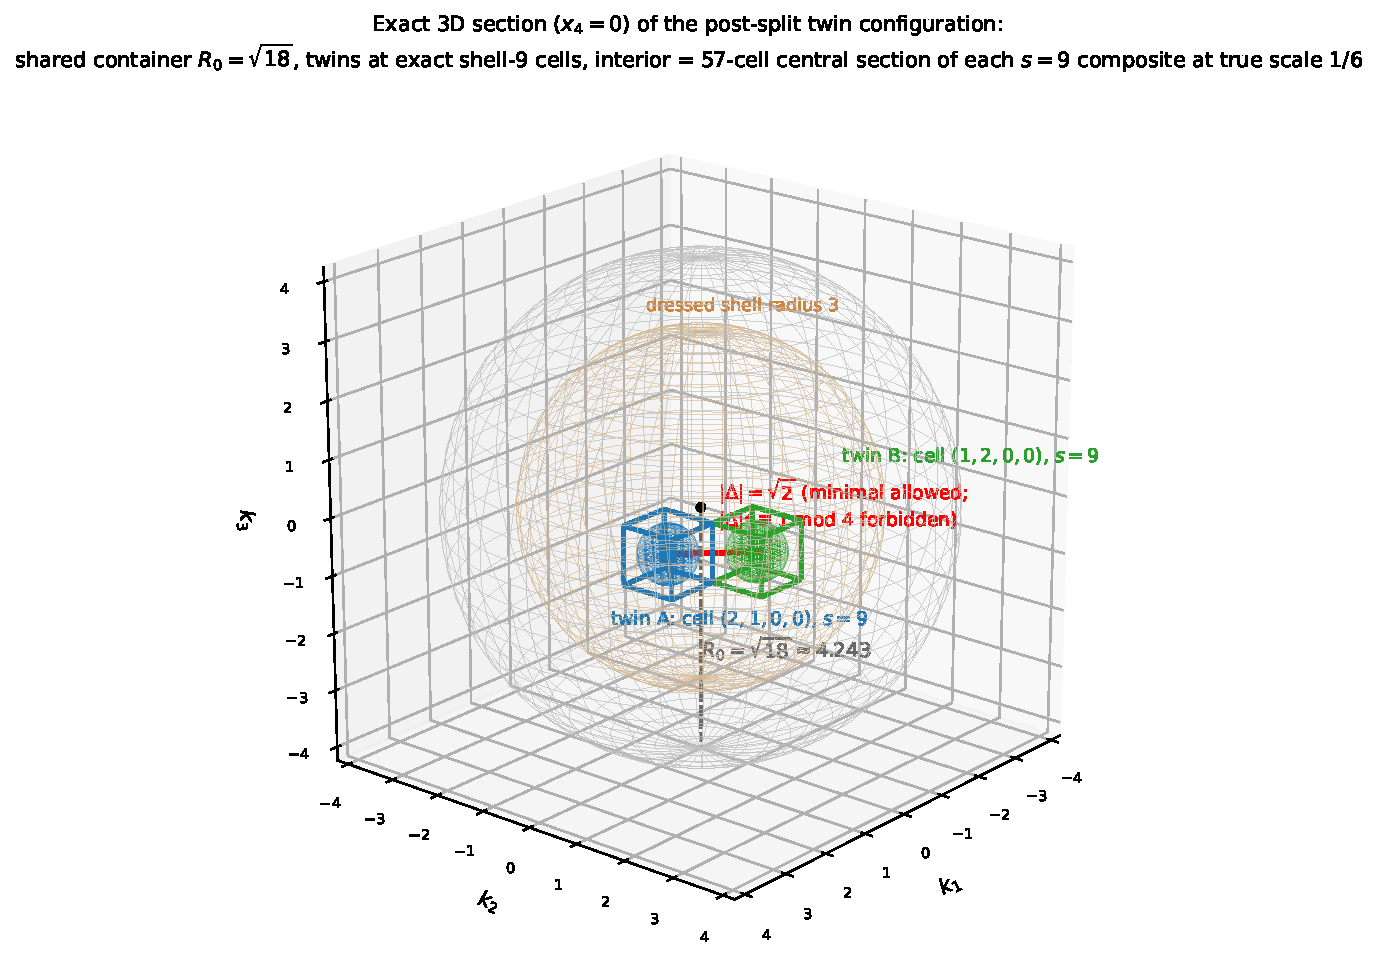
\includegraphics[keepaspectratio,alt={Figure 2. Exact 3D section of the post-split twin configuration at true scale}]{figure_paper12_2_twin_configuration.pdf}}
\caption{Figure 2. Exact 3D section of the post-split twin configuration
at true scale}
\end{figure}

\textbf{Figure 2. Exact 3-dimensional section (\(x_4=0\)) of the
post-split twin configuration.} Inside the shared container
\(R_0=\sqrt{18}\approx4.243\) (self-consistently \(R_0^2=S=18\); the
outer sphere), the twins occupy the shell-9 cells \((2,1,0,0)\) and
\((1,2,0,0)\). The separation is the minimal allowed value
\(|\Delta|=\sqrt2\) (\(|\Delta|^2=1\) is forbidden by the mod 4
selection rule). Inside the unit cell of each twin, the central
3-dimensional section (57 cubes) of the one-layer-down \(s=9\) composite
(137 cells) and its internal container (diameter 1, i.e.~\(2R_1=6\) in
internal units) are drawn exactly at scale \(1/6\). The inner sphere is
the dressed shell radius 3. All positions, separations, and scales are
exact computed values; this figure is the concretization, in the present
model, of the hierarchical state spaces of Paper 4, Figure 3.

\subsubsection{3.2 The separation spectrum and the mod 4 selection
rule}\label{the-separation-spectrum-and-the-mod-4-selection-rule}

Both twins sit on shell-9 (64 cells). Exhaustive classification of the
\(\binom{64}{2}=2016\) possible pairs yields:

\begin{itemize}
\tightlist
\item
  Allowed separations
  \(|\Delta|^2\in\{2,3,4,6,7,8,10,11,12,14,15,16,18,20\}\).
\item
  \textbf{\(|\Delta|^2\equiv1\pmod4\) (including adjacency \(1\)) is
  entirely forbidden} (by the parity structure of the two shell-9
  orbits: same-orbit pairs have even difference, mixed-orbit pairs
  \(\equiv3\pmod4\)).
\item
  The pairs decompose under \(B_4\) × swap into 18 relational classes,
  which are \textbf{completely separated} by the fringe data
  \((|\Delta|^2,|\Sigma|^2)\) alone (the inner product
  \(=(|\Sigma|^2-|\Delta|^2)/4\), so angles too can be read directly
  from the fringes).
\end{itemize}

\begin{quote}
The relative positions available to two entities with equal
representative frequencies are quantized as chord sets of
equal-frequency shells, with forbidden bands. \textbf{In this twin
system, this discrete catalogue is everything that is real (= appears in
the record) as ``distance.''}
\end{quote}

\begin{figure}
\centering
\pandocbounded{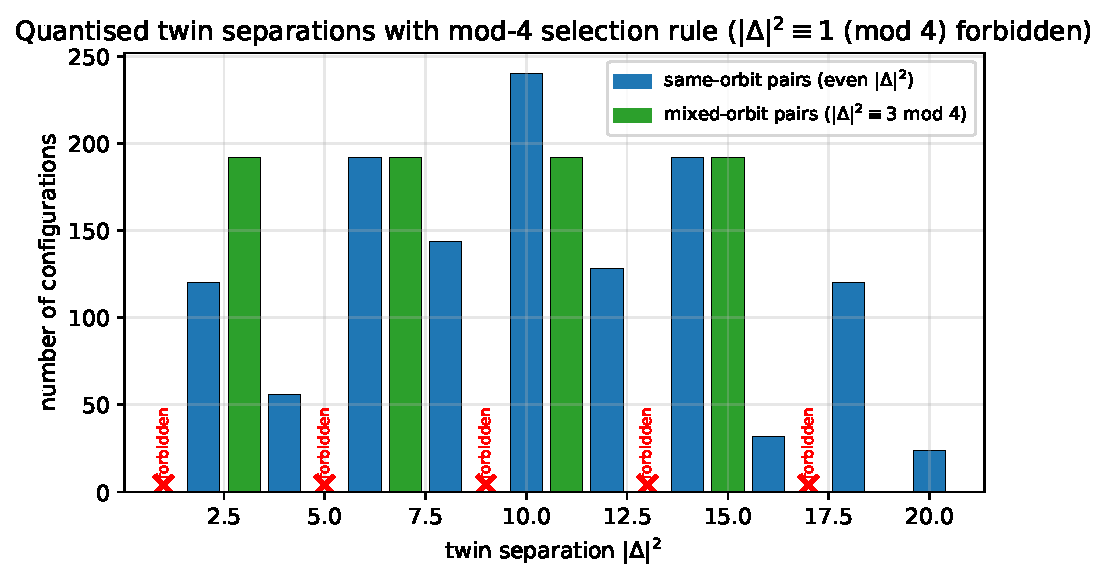
\includegraphics[keepaspectratio,alt={Figure 3. Quantised twin separations with the mod-4 selection rule}]{figure_paper12_3_separation_spectrum.pdf}}
\caption{Figure 3. Quantised twin separations with the mod-4 selection
rule}
\end{figure}

\textbf{Figure 3. Twin separation spectrum (exhaustive over 2016
configurations): \(|\Delta|^2\equiv1\ (\mathrm{mod}\ 4)\) is entirely
forbidden. Same-orbit pairs (even \(|\Delta|^2\)) and mixed-orbit pairs
(\(\equiv3\) mod 4).}

Note that since the twin system contains no \(s=1\) (DC reference), the
record is of the interferometric type (relations only), and DC = 2
directly reads off ``that there are two'' --- a minimal two-path
interferometer without a reference.

\begin{center}\rule{0.5\linewidth}{0.5pt}\end{center}

\subsection{4. The Clock Ledgers and the Status of the Schrödinger
Equation}\label{the-clock-ledgers-and-the-status-of-the-schruxf6dinger-equation}

\subsubsection{4.1 Ratios of relational
clocks}\label{ratios-of-relational-clocks}

This model has no continuous time; time is event counting (Paper 6).
Hence ``phase evolution'' is meaningful not as a function of background
time but only as \textbf{the rate at which the phase of one subsystem
advances relative to another subsystem (the clock)} (a minimal
implementation of Page--Wootters relational time {[}3{]}). There are
three candidate clocks: (i) the norm clock (\(\nu=\sqrt s\): the heavier
runs faster), (ii) the face clock (\(\nu=1/(2\sqrt s)\): the lighter
runs faster), and (iii) the bare-line clock (\(\nu=|k|\): depends on the
orbit type). Inspection yields:

\begin{itemize}
\tightlist
\item
  \textbf{The face clock is eliminated}: reading the cascade (Paper 8)
  with the face clock makes time saturate at a finite value; the only
  global clock satisfying radiation-law consistency
  (\(a\propto t^{1/2}\)) is the norm clock.
\item
  \textbf{The norm/face choice is a gauge}: the two are zero-point
  conjugate via \(\nu_{\mathrm{norm}}\nu_{\mathrm{face}}=1/2\), and the
  global flip is merely a relabeling that reciprocates all ratios. The
  non-gauge content is the single bit ``which side is additive'' --- the
  arithmetic of conservation selects the norm side, and the
  continuum-limit phase rotation law becomes \(\omega\propto\sqrt s\)
  (energy-like).
\item
  \textbf{The bare-line clock predicts a real difference}: at equal
  energy, different orbit types have different \(|k|\) (2 versus
  \(\sqrt5\) on shell-9), so \textbf{equal-energy twins beat}. The
  discriminator is precisely the mod 4 structure of §3.2 (only
  odd-\(|\Delta|^2\) classes = mixed-orbit pairs can drift), and
  discrimination requires a phase connection rule between events (§7).
\end{itemize}

\subsubsection{4.2 The Schrödinger equation is an effective
interpolation under three
conditions}\label{the-schruxf6dinger-equation-is-an-effective-interpolation-under-three-conditions}

In the limit where (i) the relational-clock subsystem has many states
(\(N\gg1\)), (ii) under censorship a single representative \(\nu\) can
represent the composite, and (iii) the discrete graining is relatively
small (\(\varepsilon\sim1/(2\sqrt s)\)), the phase ledger of event
counting becomes interpolable as a continuous-time wave equation. The
corrections are not only small, \(O(\varepsilon)\), but
\textbf{unrecordable by censorship}; at the level of records the
equation appears to hold exactly (double protection). What emerges is
the wave sector only (the analogue of a one-particle wave equation);
linear superposition across configurations (histories) does not come out
of this limit. Predicted breakdowns: few-state systems interacting with
each other, processes crossing hierarchy layers, the vicinity of
forbidden bands (Paper 9).

\begin{center}\rule{0.5\linewidth}{0.5pt}\end{center}

\subsection{5. The Exact Form of Measurement: Absence →
Presence}\label{the-exact-form-of-measurement-absence-presence}

\subsubsection{5.1 The two conditions and the cutting of the
regress}\label{the-two-conditions-and-the-cutting-of-the-regress}

Measurement requires two conditions: (1) interacting with the system;
(2) knowing that the state has changed. Condition (2) requires knowledge
of the prior state, which is itself a measurement, hence an infinite
regress --- the only possible detection is \textbf{absence becoming
presence}. In this model, this analysis becomes a theorem as it stands:

\begin{enumerate}
\def\labelenumi{\arabic{enumi}.}
\tightlist
\item
  Before an event the interior of a composite is a cloud by censorship,
  and a record of the prior state is \textbf{absent in principle} (there
  is no ledger to compare against).
\item
  The \(\lambda\) ledger is \textbf{append-only} (exact monotonic
  increase of \(\Sigma\lambda^2\), Paper 6). Only one kind of
  transaction exists in the ledger --- the append: absence → presence.
\end{enumerate}

\begin{quote}
\textbf{Exact form of measurement}: a measurement is an append event to
the \(\lambda\) ledger. ``Collapse'' is the appearance of a record, and
its irreversibility reduces to the same single bit as the arrow of time
(one postulate fewer). The arbitrariness of the location of the
Heisenberg cut corresponds to the boundary of hierarchical jurisdiction
(defined by censorship). This is consistent with the fact that all real
measurements terminate in counts of appearances (clicks, grains on a
plate) {[}5{]}.
\end{quote}

\subsubsection{5.2 Explicit computation of the first
measurement}\label{explicit-computation-of-the-first-measurement}

Across the decay of twin A, \(9\to(5,3,1)\): DC (fragment count)
\(2\to4\); record lines \(2\to9\) (9 appear, 2 disappear);
\(\Sigma\lambda^2=2/9\to74/45\) (exact increase); \(\Sigma\nu^2=18\)
(conserved). Decisive is the promotion of the information class: with
the appearance of \(s=1\) = the reference wave, the record changes from
the interferometric type to the \textbf{holographic type} (full
configuration recoverable, Paper 7 §6.5; reconstruction by a reference
wave is a structural correspondence with Gabor's holography {[}15{]}).
\textbf{In this system the first decay and the first measurement are the
same event, and the measuring apparatus (the reference wave) is
generated by the event itself.} Note that the disappeared lines ``leave
nothing to read'' --- an existing record can be read now, but the
detection of a disappearance requires the earlier record and regresses.
This is why only appearances are readable, asymmetrically.

\begin{figure}
\centering
\pandocbounded{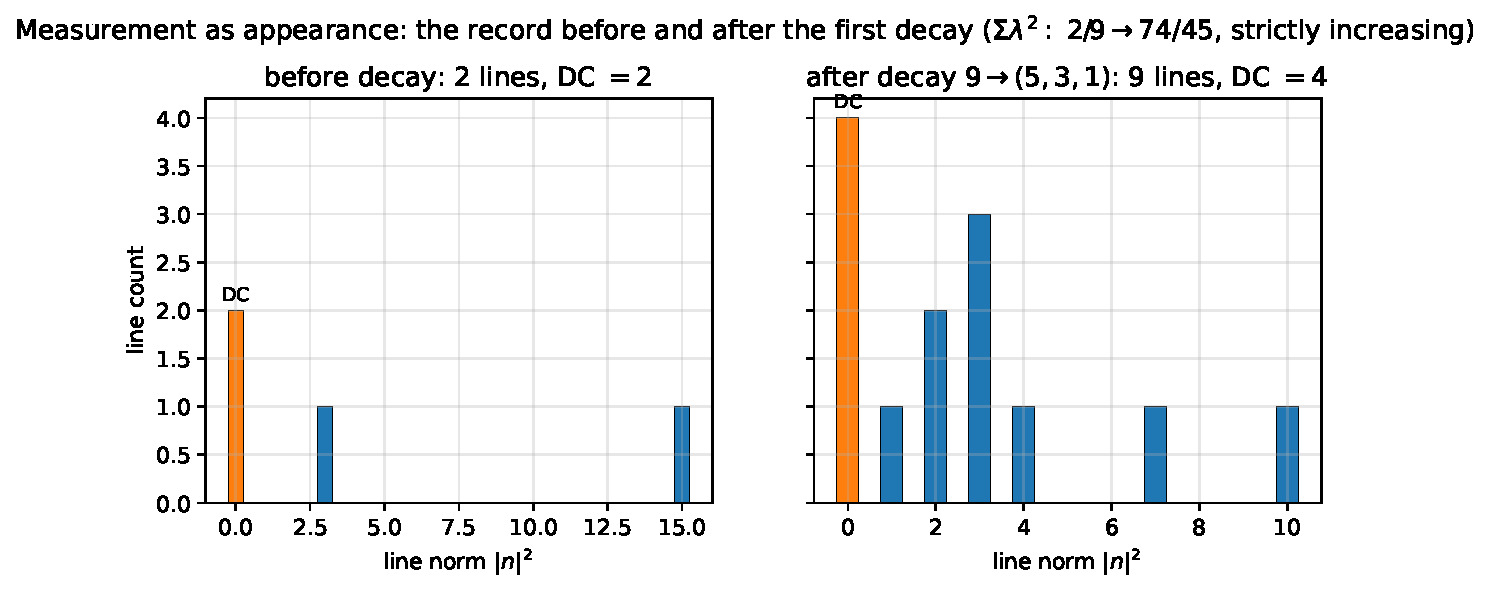
\includegraphics[keepaspectratio,alt={Figure 4. Measurement as appearance: the record before and after the first decay}]{figure_paper12_4_measurement.pdf}}
\caption{Figure 4. Measurement as appearance: the record before and
after the first decay}
\end{figure}

\textbf{Figure 4. Measurement = appearance: the record lines before and
after the first decay \(9\to(5,3,1)\). DC (fragment count) goes
\(2\to4\), the lines \(2\to9\), and \(\Sigma\lambda^2\) increases
exactly from \(2/9\) to \(74/45\).}

Note that the representative configuration of this section (\(v_3=e_3\))
is one example under equal weighting; if the record continuity rule of
§7.1 is adopted as the vertex rule, it is redrawn with licensed
configurations (\(v_3=\pm e_1\) etc. for parents of type \((2,1,0,0)\)).
The conclusions of this section --- the DC increment, the exact increase
of \(\Sigma\lambda^2\), and the holographic promotion --- are robust
against the choice of configuration.

\subsubsection{5.3 Measure bifurcation}\label{measure-bifurcation}

Comparing the final-state statistics of the two-stage twin decay in
exact rationals: one-shot (equal weight over final configurations) gives
\(P=60/61=0.98361\), sequential (conditional counting) gives
\(396/403=0.98263\), equal weight over paths gives \(0.96000\) ---
\textbf{they do not agree} (one-shot versus sequential difference
\(+0.00098\)). The timeless counting principle alone does not fix the
measure uniquely; the ``factual structure of the event'' (one-shot or
sequential) produces an observable difference. Standard theory possesses
no derived answer to this question (the operational rule --- sequential
if the intermediate is recorded, path sum if not --- has an underived
boundary, namely the cut {[}5,6{]}); in this model, ``the presence or
absence of a record selects the composition rule'' is a candidate answer
with the prospect of being derivable (because the record is a
theorem-level concept).

\begin{center}\rule{0.5\linewidth}{0.5pt}\end{center}

\subsection{6. Layer Resolution of
Entanglement}\label{layer-resolution-of-entanglement}

\subsubsection{6.1 The relational-only readout
theorem}\label{the-relational-only-readout-theorem}

The self-spectrum of a single fragment (the self-term of the intensity)
lies on \textbf{all-components-even} vectors with components
\(\{0,\pm2k_i\}\). A nonzero even component does not belong to the
logical-wave alphabet \(\{0,\mathrm{odd}\}\), so \textbf{self lines are
identically invisible in the odd (logical-wave) sector}. As a corollary,
what a logical-wave decoder can read from the twin system is only the DC
(counts) and the odd-visible cross lines (relations) --- individuals
cannot be read. Moreover, same-orbit pairs have even cross lines as
well; the relations readable in the odd sector are limited to
mixed-orbit pairs (\(|\Delta|^2\equiv3\bmod4\)).

\subsubsection{6.2 The distance-independent conditional shift and
no-signalling}\label{the-distance-independent-conditional-shift-and-no-signalling}

B's branching statistics after A's decay (exact rationals):
\((0.774,0.226)\) with A undecayed, \((0,1)\) after A\(=(5,3,1)\),
\((0.923,0.077)\) after A\(=(3,3,3)\) (total variation 0.774). This
shift is due to the \textbf{global constraint} that the origin slot
\(c(1)=1\), and \textbf{does not depend on the lattice separation of the
twins at all}. The influence does not propagate through the space of the
child layer --- the event is a single append at ``the level where the
two are not separated,'' and \textbf{instantaneity is not a claim about
speed but a statement about category}.

No-signalling: under the sequential measure B's marginal statistics
depend on the order, but the order and the attribution (which came
first; which produced what) do not exist in the final record.
\textbf{Order-dependent quantities are ledger quantities that cannot be
read out, and operational no-signalling is a consequence of the record
structure (attribution censorship).}

\subsubsection{6.3 Parity protection and the isomorphism to two-path
interference}\label{parity-protection-and-the-isomorphism-to-two-path-interference}

Since \(S=18\) is even and has no single-state slot, \textbf{an
entangled pair cannot become ``one particle'' no matter how coarsely it
is viewed from layers above} --- pair and particle are arithmetically
distinguished, different kinds of objects (parity protection).

The same map applies to two-path interference of a single wave packet:
interference is a phase beat of a real wave (§2.2) and requires no
superposition of histories; detection is an append event one layer up;
and the ``instantaneous vanishing of the distant lobe'' is not a process
in the child layer. The EPR two-particle case and the double-slit
one-particle case are two appearances of the same structure: ``one
object at the layer above is spread over two places in its own layer.''

Note that this mechanism is a global (nonlocal) hidden structure, lying
outside the local-hidden-variable premises forbidden by Bell's theorem
{[}7{]}. The correlations verified so far (channel anticorrelation) are
those of a single observable; a CHSH-type test {[}8{]} would require
constructing an analogue of the choice of measurement settings (not
constructed; not claimed).

\begin{center}\rule{0.5\linewidth}{0.5pt}\end{center}

\subsection{7. Vertex Deficits and the Two Hidden
Axes}\label{vertex-deficits-and-the-two-hidden-axes}

\subsubsection{7.1 Derivation of the vector conservation law and the
one-unit
deficit}\label{derivation-of-the-vector-conservation-law-and-the-one-unit-deficit}

We exhaustively inspected whether the event rule (the vertex map) closes
with the existing inventory alone, in the minimal form of the record
continuity rule --- that the parent's identity line vector \(v_9\)
persists in the intensity spectrum (cross lines) of the daughter system.
Results:

\begin{itemize}
\tightlist
\item
  The persistence condition is \(v_5\pm v_3=\pm v_9\), that is,
  \textbf{conservation of the vector sum of cell positions (a momentum
  analogue)} is derived without postulate. For parents of type
  \((2,1,0,0)\) (48 cells) solutions exist, 4 per cell (residual
  \(Z_2\times Z_2\)).
\item
  The \((3,3,3)\) channel has zero persistence solutions on every cell
  (identity-erasing type) --- aligning with the
  holographic/interferometric dichotomy (§5.2).
\item
  \textbf{Parents of type \((1,1,1,1)\) (16 cells) cannot preserve the
  line in any allowed channel.} The deficit is exactly one unit in two
  equivalent accountings: the support of the daughter pair is at most 3
  axes \(<\) 4 axes (one axis short), and the minimal line-preserving
  splitting \((5,5)\) has \(s=10=9+1\) (one zero-point quantum short).
\end{itemize}

\subsubsection{7.2 A second, independent
deficit}\label{a-second-independent-deficit}

Inspecting the endpoint bookkeeping of the excitation degree
\(\varepsilon(k)=(-1)^{\Sigma|k|}\) (Paper 10) over all parent orbits ×
all channels × all daughter orbits for \(s=7\)--\(13\): the
\((1,1,1,0)\) type at \(s=7\) and the \((1,1,1,1)\) type at \(s=9\)
\textbf{cannot conserve \(\varepsilon\) under any assignment}.
\(\varepsilon\) conservation is equivalent to conservation of bare norm²
parity \(\Sigma|k_d|^2\equiv|k_p|^2\pmod2\), and it is a ledger
\textbf{independent} of line closure (§7.1) --- all four combinations
are realized.

\subsubsection{7.3 The licensing principle for virtual displacements and
cubic
vertices}\label{the-licensing-principle-for-virtual-displacements-and-cubic-vertices}

That the visible four-axis ledgers carry two independent one-unit
deficits indicates the existence of \textbf{two invisible directions}: R
on the curvature/energy side (deficit unit = one s quantum) and Q on the
bare-parity side (deficit unit = one \(Z_2\) bit). The mod 8 theorem
(Paper 11) requires only that the visible (integer-ledger) sector have 4
axes and does not restrict the number of background axes --- consistent
with the reading of a subjective 4 dimensions over a 6-axis background
(\(xyzt\) + \(R\) + \(Q\)).

Invisible directions are not recorded. Since there is no fact about an
unrecorded difference (the record theorem), \textbf{intermediate
displacements along the invisible directions (virtual states) violate no
visible ledger} --- the licensing of virtual states becomes a
consequence of the record theorem rather than an ad hoc rule. At the
endpoints (recorded configurations) all visible ledgers hold (the
displacement is repaid to net zero). Under this licence, two-body
splittings forbidden by parity violation in the visible ledgers become
virtually unlocked, and \textbf{every decay decomposes into sequences of
cubic vertices} (12 paths for \(9\to(5,3,1)\), 2 paths for
\(9\to(3,3,3)\), virtual intermediate states
\(\{(1,7),(1,9),(3,5),(3,7),(5,5)\}\)). The skeleton of a path sum ---
multiple paths to the same final state --- appears at the level of
amplitude-free counting {[}12{]}. The picture in which hidden dimensions
carry charge-like structure corresponds structurally to Kaluza--Klein
{[}13,14{]} (no identification is made).

An exhaustive inspection of the chain of custody (at each step the
splitter's line passes into the daughters' cross lines) shows that
parents of type \((2,1,0,0)\) possess 68 fully continuous paths while
parents of type \((1,1,1,1)\) possess zero --- their identity can only
pass through the invisible sector. Decays divide into two classes: the
\textbf{reconstructible type} (the parent can be reconstructed from the
daughters' cross lines: the structural correspondence of invariant-mass
peaks) and the \textbf{missing-information type} (full reconstruction
from the visible final state is impossible in principle: the structural
correspondence of decays with missing energy).

\begin{center}\rule{0.5\linewidth}{0.5pt}\end{center}

\subsection{8. Discussion: The Transport Principle and Candidate
Answers}\label{discussion-the-transport-principle-and-candidate-answers}

\subsubsection{8.1 The transport
principle}\label{the-transport-principle}

A theorem of standard theory holds in this model as well whenever all of
its premises have counterparts among the axioms of this model
(\(\nu\lambda=1\) = invariant speed and null structure, the zero point,
the asymmetric bit) or its verified structures (lattice gauge
kinematics, quantum statics, the grammar of perturbation theory,
measurement theory, the skeleton of probability). Theorems whose
premises touch the differences (continuous spacetime, amplitude
linearity, unitary evolution --- each of which is a censored
approximation in this model) hold only within the validity domain of the
approximation. For the structures that standard theory settled by
\textbf{postulate} (the \((1,3)\) signature, the choice of gauge group,
the existence of matter fields), the connection is complete provided the
qualification to adopt corresponding axioms, theorems, or equivalent
inputs is in place; their \textbf{derivation} is a research direction in
which this model could go beyond standard theory (not re-deriving them
is not a defect).

\subsubsection{8.2 Status of answers to questions standard theory leaves
unanswered}\label{status-of-answers-to-questions-standard-theory-leaves-unanswered}

Questions to which the computations of this model give answers (or
candidate answers): the measurement problem (collapse = append), the
location of the cut (the boundary of hierarchical jurisdiction), the
problem of time (event counting and one bit), the coexistence of
unitarity and collapse (two phases of one structure), the selection of
dimension (censorship ceiling + mod 8 + self-duality), the compatibility
of a discrete foundation with unbroken Lorentz symmetry (the breaking is
censored), the boundary of composition rules (the presence or absence of
a record selects --- candidate), the origin of the Born rule (record =
intensity + counting --- candidate).

\subsubsection{8.3 Falsifiability}\label{falsifiability}

\begin{enumerate}
\def\labelenumi{(\roman{enumi})}
\tightlist
\item
  \textbf{Gravitationally mediated entanglement}: in this model
  amplitudes cannot couple to curvature (Paper 9), so BMV-type
  experiments {[}10,11{]} are a live arbiter. (ii) \textbf{Measure
  bifurcation} (\(\sim10^{-3}\)): the difference of event structure is
  in principle observable as a difference of branching statistics. (iii)
  The stable-species structure, the two decay classes, and the mod 4
  selection rule are exact predictions exhaustively verified within the
  model (conversion to physical units requires cross-validation through
  independent dimensionless observables and is outside the scope of this
  paper).
\end{enumerate}

\begin{center}\rule{0.5\linewidth}{0.5pt}\end{center}

\subsection{9. Scope of Claims of This
Paper}\label{scope-of-claims-of-this-paper}

What this paper claims: (1) The three ledgers and the identity
\(\nu_0R'=1/2\), the readout of energy as comb spacing, the
minimal-uncertainty wave packet. (2) Pair creation forced by parity, the
separation spectrum and the mod 4 selection rule, the complete
separation of relational classes by fringes. (3) The single gauge bit of
clocks and the elimination of the face clock, the status of the
Schrödinger equation as an effective interpolation under three
conditions. (4) Measurement = append, the dissolution of collapse,
measure bifurcation (exact values). (5) The relational-only readout
theorem, the distance-independent shift, no-signalling = attribution
censorship, parity protection. (6) The derivation of the vector
conservation law, the two independent one-unit deficits, the licensing
principle for virtual displacements, the cubic-vertex decomposition, the
two classes of decay.

What this paper does not claim: (1) Identification with the real
universe or real particles (the language of structural correspondence is
maintained throughout). (2) Violation or non-violation of Bell
inequalities (an analogue of setting choice is not constructed). (3)
Finite coupling constants or transition rates (the dynamics of the
vertex map is not constructed). (4) A complete formulation of the 6-axis
background (the existence proof of the invisible directions is the
discovery of deficits, not a construction). (5) Theorem-level status for
the Born rule or the composition rule (left as candidate answers).

\begin{center}\rule{0.5\linewidth}{0.5pt}\end{center}

\subsection{10. Conclusion}\label{conclusion}

In the twin minimal space model, the skeleton of quantum-looking
behavior --- wave packets and the saturation of uncertainty, discrete
detection and irreversibility, distance-independent correlations and
no-signalling, virtual states and vertex structure --- was derived as a
\textbf{reading of hierarchy interfaces of a discrete relational model},
without assuming amplitudes, continuous time, or collapse of the wave
function. What remains are the constructive tasks that have converged
onto a single object --- the factual structure of the event (settling
the measure, the phase connection rule, the analogue of setting choice)
--- and the formulation of the two invisible directions. The relation to
standard theory is ``the same results under a different map,'' and all
differences have been made explicit in falsifiable form.

\begin{center}\rule{0.5\linewidth}{0.5pt}\end{center}

\subsection{Appendix: Key Points of the Reproduction
Procedure}\label{appendix-key-points-of-the-reproduction-procedure}

The three-ledger spectra (exact coefficients of structure factor ×
sinc), the twin catalogue (\(B_4\) × swap canonicalization of the
\(\binom{64}{2}=2016\) pairs), the before/after comparison of the first
measurement (line sets, \(\Sigma\lambda^2\)), the exact rational
comparison of the three measures, the line classification for the
relational-only readout, the exhaustive inspection of vertex closure and
\(\varepsilon\) bookkeeping (\(s\le13\)), and the full enumeration of
cubic-vertex paths. Scripts and research notes are provided in the
public repository (https://github.com/WurabeSeiji/ai-chat-logs-open).

\begin{center}\rule{0.5\linewidth}{0.5pt}\end{center}

\subsection{References}\label{references}

{[}1{]} Noriaki Kihara, Paper 4, v1.0, 2026. Concept DOI:
10.5281/zenodo.20638962.

{[}2{]} Noriaki Kihara, Papers 5--11, v0.2, 2026. (this series) (Paper 5: 10.5281/zenodo.20640454; Paper 6: 20640456; Paper 7: 20640458; Paper 8: 20640460; Paper 9: 20640462; Paper 10: 20640464; Paper 11: 20640466)

{[}3{]} D. N. Page and W. K. Wootters, ``Evolution without evolution,''
Physical Review D 27 (1983), 2885--2892.

{[}4{]} J. A. Wheeler, ``Information, physics, quantum: The search for
links,'' in \emph{Complexity, Entropy and the Physics of Information},
Addison-Wesley, 1990.

{[}5{]} J. von Neumann, \emph{Mathematische Grundlagen der
Quantenmechanik}, Springer, 1932.

{[}6{]} W. H. Zurek, ``Decoherence, einselection, and the quantum
origins of the classical,'' Reviews of Modern Physics 75 (2003),
715--775.

{[}7{]} J. S. Bell, ``On the Einstein Podolsky Rosen paradox,'' Physics
1 (1964), 195--200.

{[}8{]} J. F. Clauser, M. A. Horne, A. Shimony, and R. A. Holt,
``Proposed experiment to test local hidden-variable theories,'' Physical
Review Letters 23 (1969), 880--884.

{[}9{]} R. Penrose, ``On gravity's role in quantum state reduction,''
General Relativity and Gravitation 28 (1996), 581--600.

{[}10{]} S. Bose et al., ``Spin entanglement witness for quantum
gravity,'' Physical Review Letters 119 (2017), 240401.

{[}11{]} C. Marletto and V. Vedral, ``Gravitationally induced
entanglement between two massive particles is sufficient evidence of
quantum effects in gravity,'' Physical Review Letters 119 (2017),
240402.

{[}12{]} R. P. Feynman, ``Space-time approach to non-relativistic
quantum mechanics,'' Reviews of Modern Physics 20 (1948), 367--387.

{[}13{]} T. Kaluza, ``Zum Unitätsproblem der Physik,'' Sitzungsber.
Preuss. Akad. Wiss. Berlin (1921), 966--972.

{[}14{]} O. Klein, ``Quantentheorie und fünfdimensionale
Relativitätstheorie,'' Zeitschrift für Physik 37 (1926), 895--906.

{[}15{]} D. Gabor, ``A new microscopic principle,'' Nature 161 (1948),
777--778.

\begin{center}\rule{0.5\linewidth}{0.5pt}\end{center}

\subsection{License}\label{license}

This paper is published under CC BY 4.0.\\
Reuse, adaptation, translation, and citation are permitted, provided
that the author name, version, publication date, and source are clearly
indicated.

\end{document}
